\newcommand{\orgmode}{\texttt{org-mode}}
\newcommand{\Makefile}{\mintinline{shell}{Makefile}}
\newcommand{\context}{\mintinline{shell}{context}}
\newcommand{\CC}{C\nolinebreak\hspace{-.05em}\raisebox{.4ex}{\tiny\bf +}\nolinebreak\hspace{-.10em}\raisebox{.4ex}{\tiny\bf +}}
\def\CC{{C\nolinebreak[4]\hspace{-.05em}\raisebox{.4ex}{\tiny\bf ++}}}

\section{Summary of report D1.1}


\Ac{QMCkl} aims at providing a high-performance
implementation of the main kernels of \ac{QMC} methods. 
\ac{WP}~1 focuses on defining the \ac{API}, the tests,
and a \emph{pedagogical} presentation of the main algorithms.
In \ac{WP}~3, the \ac{HPC} experts use this repository as a reference for re-writing
optimized versions of the functions proposed in this pedagogical version of the library.

To maximize the portability to unknown architectures, we have chosen to provide an \ac{API} which
is compatible with the C programming language. The foundations of the library are written in C, but Fortran
was chosen to express the kernels as it is more convenient than C for expressing linear algebra.
The dependencies to external software are kept minimal to facilitate the installation, and the
BSD 3-clause license was chosen to facilitate the adoption of the library by industrial 
collaborators.

As this version version of the library is intended to be mostly used as documentation, 
we chose to use literate programming\cite{knuth_1992} in {\orgmode}
format.\cite{schulte_2012,orgmode} The documentation
is first written, and the code illustrates the documentation. From the same source files,
the documentation is generated both in text and HTML formats, as well as the C code of the library.
This practice helps the documentation to always be consistent with the code.


\hline

The documentation of the current status of the library is available
at \url{https://trex-coe.github.io/qmckl}, and the source code is
available on the GitHub repository at \url{https://github.com/trex-coe/qmckl}.


\section{Work done since D1.1}

% Autotools
%    Removed munit
%    Facilitates packaging (.deb for trexio)
%    Package for Spack, not upstream yet

% Integration of TREXIO

% New kernels
%    AOs
%    MOs
%    Jastrow mu?

% Feedback from HPC experts
%   Data structures for HPC
%   QMCkl dgemm => BLAS


% Feedback from users
%   Edgar and fixed number of points
%   PoC: integration in CHAMP

% Python interface
%    Adoption in TREXIO tools
%    Possible collaboration with industry => DFT code

\subsection{Algorithms}

Some users will run calculations using as a trial wave function a
single determinant with thousands of electrons, and some other users
will run calculations with a small number of electrons but with millions
of Slater detrminants. These two different profiles impose that the
library has to be efficient both in the regime of small and large numbers
of electrons. When the number of electrons is large, interactions
become local and linear-scaling algorithms can be introduced. However,
such algorithms become inefficient for small sizes.  Hence, to
satisfy these two regimes, multiple algorithms will be implemented to
achieve the same task, and the library will decide at run time which
algorithm should use to minimize the time to solution.


\subsection{Dependencies}

Dependencies in other software components is a critical point that
should be considered seriously. If a user is not able to install the
required external libraries and tools, the user is not going to be
able to use our library. So the list of external dependencies should
be kept as small as possible.  External libraries should be used
\emph{only} if their use is strongly justified, and if we are sure
that the users will be able to have access to them.

The dependencies needed to use pre-compiled versions of the library
are \ac{BLAS} and \ac{LAPACK}.

The dependencies needed to compile the code are
a C and a Fortran compiler, GNU make, \ac{BLAS} and \ac{LAPACK}, and
$\mu$nit\cite{munit} for building the unit tests.

The dependencies needed to create the \ac{HTML} documentation are
Emacs~26 and the package Emacs-htmlize.

\subsection{Packaging}

We intend to use the GNU build system, Autotools,\cite{autotools} for
configuration and installation scripts.
Although there exists more modern build tools, we have chosen a
solution that will be easy for the end user, and which is one of the
most reliable in terms of portability among different architectures.

In the future, we plan to provide \texttt{.deb} and \texttt{.rpm}
packages for the most common Linux distributions, as well as a package
for the Spack package manager\cite{spack}.


\subsection{Continuous integration}

Continuous integration has been setup on the GitHub platform. Upon
receiving a pull request, the repository is automatically cloned on a virtual machine. The source code is then extracted from the {\orgmode}
files and the library is compiled. Then the unit tests are compiled
and linked together with the library. If all the tests pass, the
pull request is considered valid, and can be merged.

When the code is updated, the documentation is automatically built and
the server hosting the documentation is updated, such that the web
site containing the documentation is always synchronized with the
latest version of the master branch of the GitHub repository.


\section{Source code}

\subsection{Choice of the programming language}

\subsection{License}

The library is licensed under the open-source 3-clause BSD license to facilitate
its adoption in all quantum chemistry software, commercial or not.

\clearpage
\section{Design of the library}

The proposed \ac{API} should allow the library to deal with memory
transfers between CPU and accelerators, and to use dynamically
different levels of floating-point precision.  We chose a
multi-layered design with low-level and high-level functions (see
below).

\subsection{Naming conventions}

To avoid namespace collisions, we use \mintinline{C}{qmckl_} as a prefix for
all exported functions and variables.  All exported header files
should have a file name prefixed with \mintinline{shell}{qmckl_}.

For instance, if the name of the {\orgmode} file is
\mintinline{shell}{xxx.org}, the name of the produced C files should
be \mintinline{shell}{xxx.c} and \mintinline{shell}{xxx.h} and the
name of the produced Fortran file should be
\mintinline{shell}{xxx.f90}

Arrays are in uppercase and scalars are in lowercase.

In the  names of  the variables and  functions, only the singular
form is allowed.

\subsection{Application programming interface}

In the C language, the number of bits used by the basic integer types
(\mintinline{C}{int}, \mintinline{C}{long int}, \textit{etc}) can
change from one architecture to the other. To circumvent this
problem, we choose to use the integer types defined in
\mintinline{C}{<stdint.h>} where the number of bits used to represent
integers are fixed.

To ensure that the library will be easily usable in \emph{any} other
language than C, we restrict the data types in the interfaces to the
following:
\begin{itemize}
\item 32-bit and 64-bit integers, scalars and and arrays
  (\mintinline{C}{int32_t} and \mintinline{C}{int64_t})
\item 32-bit and 64-bit floats, scalars and and arrays
  (\mintinline{C}{float} and \mintinline{C}{double})
\item Pointers are always casted into 64-bit integers, even on legacy 32-bit architectures
\item ASCII strings are represented as a pointers to character arrays
  and terminated by a zero character (C convention).
\item Complex numbers can be represented by an array of 2 floats.
\item Boolean variables are stored as integers, \mintinline{C}{1} for
\mintinline{C}{true} and \mintinline{C}{0} for \mintinline{C}{false}
\item Floating point variables should be by default
\mintinline{C}{double}, unless explicitly mentioned
\item integers used for counting should always be \mintinline{C}{int64_t}
\end{itemize}

To facilitate the  use in other languages than C, we plan to provide 
bindings for other languages.


\subsubsection{Global state}

Global variables should  be avoided in the library,  because it is
possible that one  single program needs to  use multiple instances
of the library, or to use the library in a multi-threaded context.
To solve this  problem we propose to use a pointer
to a {\context}  variable,  built   by  the  library   with  the
\mintinline{C}{qmckl_context_create} function. The
{\context} contains the global state of the library, and is used as
the first argument of most \ac{QMCkl} functions. Thread safety is 
implemented in critical functions of the context with a
\texttt{pthreads} lock, to provide a simple and general locking
mechanism.

The internal structure of the {\context}  is not specified, to give a
maximum of  freedom to  the different  implementations.  Modifying
the  state   is  done   by  setter   and  getter functions,   prefixed  by
\mintinline{C}{qmckl_context_set_}  an
\mintinline{C}{qmckl_context_get_}.
When a {\context} variable is modified by a setter, a copy of the old
data structure is made and updated, and the pointer to the new data
structure is returned, such that the old contexts can still be
accessed in case they are already involved in running computations by
other threads. It is also possible to modify the state in an mutable
fashion, using the \mintinline{C}{qmckl_context_update_} functions,
although it is not recommended as the default practice.
The {\context} and its old versions can be destroyed with
\mintinline{C}{qmckl_context_destroy}.


\subsubsection{Low-level functions}

Low-level functions are very simple functions which are leaves of
the function call tree (they don't call any other \ac{QMCkl} function).
These  functions   are   \emph{pure} (i.e. without side effects), and
unaware of the \ac{QMCkl} {\context}. They are not allowed to
allocate/deallocate memory, and if they need temporary memory it
should be provided in input. This will prevent a degradation of
performance due to unnecessary repeated memory allocations and
deallocations hot spots of the programs.


\subsubsection{High-level functions}

High-level functions  are higher in the function  call tree.
They  are  able  to  choose which  lower-level  function  to  call
depending on the required precision, and to do the corresponding type
conversions. They are also able to choose between different algorithms
(sparse or dense for example), according to parameters defined in the
{\context}.  These functions are also responsible for allocating
temporary storage, to optimize the use of accelerators.

The high-level functions should be pure, unless if it is
justified. If any, all the side effects should be made in the
\texttt{context} variable.

\subsubsection{Numerical precision}

The number of bits of precision  required for a function should be
given as an input of low-level computational functions. This input
will be used to define the values of the different thresholds that
might be used to avoid computing unnecessary numerical
noise. High-level functions will use the precision specified in the
\texttt{context} variable.


\section{Codesign}
\label{sec:codesign}

Research codes are developed over a long period of time by multiple
researchers, Ph.D students and post-docs. The professional evaluation
of these people is based on their scientific production and not on the
quality of the software they write, so code quality and refactoring is
often left in the low-priority task queue. As a consequence, research
codes often depend on some choices made at an immature stage of the
program, and solutions to bypass the wrong choices make the code
complicated to understand for external programmers, especially if they
are not familiar with the domain.

\subsection{Kernel extraction}

The strategy we have chosen to extract the kernels of the codes is to
first discuss among the developers of \ac{QMC} codes to understand how they have
implemented each particular kernel. Once the developers have agreed on
which algorithm is best, they first formulate the algorithm in terms
of mathematical expressions in a {\LaTeX} file, and they create a prototype application 
(the \emph{mini-application}) implementing \emph{only} the kernel of
interest. This mini-application can be easily compiled and executed,
and is considered valid when it reproduces exactly the values obtained
with the kernel present in the original \ac{QMC} code.

The mini-application is then thoroughly modified together with the
\ac{HPC} experts involved in \ac{WP}3 until the optimal data
structures and algorithms are determined. This step is crucial to
facilitate the access to performance in the \ac{HPC} versions of the
library that will be developed in \ac{WP}3.  Once the \ac{QMC} and
\ac{HPC} specialists have agreed on the data structures, the kernel is
ready to be implemented in the
library.


\subsection{A concrete example}

The first kernel we have been working on is the three-body component of
the Jastrow factor, which is one of the potential bottlenecks of
extreme-scale calculations that will run on exascale machines.
In the CHAMP program, it is expressed as

\newcommand{\Jeen}{J_{\text{een}}}
\newcommand{\Nel}{N_{\text{elec}}}
\newcommand{\Nat}{N_{\text{nucl}}}
\newcommand{\Nord}{N_{\text{nord}}}
\newcommand{\lmax}{p-k-2\delta_{k,0}}
\newcommand{\br}{\mathbf{r}}
\newcommand{\bR}{\mathbf{R}}
\[
  \Jeen (\br,\bR) = \sum_{\alpha=1}^{\Nat} \sum_{i=1}^{\Nel} \sum_{j=1}^{i-1}
\sum_{p=2}^{\Nord} \sum_{k=0}^{p-1}
\sum_{l=0}^{\lmax} c_{lkp\alpha}
\left( {r}_{ij} \right)^k
\left[ \left( {R}_{i\alpha} \right)^l + \left( {R}_{j\alpha} \right)^l \right]
\left( {R}_{i\,\alpha} \, {R}_{j\alpha} \right)^{(p-k-l)/2} 
\]
where
$\Nel$ is the number of electrons, 
$\Nat$ is the number of nuclei,
$\Nord$ is the maximum order of the polynomial, 
$\br$ contains rescaled electron-electron distances, 
$\bR$ contains rescaled electron-nucleus distances,
and $c_{lkp\alpha}$ are the variational parameters which are non-zero
only when $p-k-l$ is even.

For \ac{QMC} simulations, the first and second derivatives of $\Jeen$ with
respect to the electron coordinates are also required. To optimize the
parameters, the derivative with respect to $c_{lkp\alpha}$
should also be available, and in the context of molecular dynamics or
geometry optimization the first derivatives with respect to $\bR$ are
also required. To compute these derivatives, multiple intermediates
will be common and we need to identify them such that the same
intermediates can be reused for several derivatives.

We have written a mini-application to implement the three-body component
of the Jastrow factor, as well as the first and second derivative with
respect to electron coordinates. This mini-application, available on
GitHub\footnote{\url{https://github.com/trex-coe/irpjast}} has allowed us to
rewrite the expressions in a way allowing us to take advantage of BLAS3
matrix multiplications. The formula is now expressed in terms of
rank-3 and rank-4 tensors
\newcommand{\tr}{\, \bar{\mathtt{r}}}
\newcommand{\tR}{\, \bar{\mathtt{R}}}
\newcommand{\tP}{\, \bar{\mathtt{P}}}
\[
  \Jeen(\br,\bR) = 
  \sum_{p=2}^{\Nord}\sum_{k=0}^{p-1}
  \sum_{l=0}^{\lmax} 
    \sum_{\alpha=1}^{\Nat}
    c_{lkp\alpha}
    \sum_{i=1}^{\Nel}
    {\tR}_{i,\alpha,(p-k-l)/2}\,
  {\tP}_{i,\alpha,k,(p-k+l)/2}
  \]
with 
  \[
  {\tP}_{i, \alpha, k, l} = \sum_{j=1}^{\Nel} {\tr}_{i,j,k}\,{\tR}_{j,\alpha,l}.
  \]
  
Similarly, the gradient with respect to electron coordinates and the
Laplacian require an additional intermediate array and reuses ${\tP}$. As
the gradient ($\nabla_{i}$) and the Laplacian ($\Delta_i$) have a
large part of their expression in common, the $3\Nel$ components of
the gradient and the $\Nel$ components of the Laplacian are stored in
the same array, adding an extra index $m=(1,2,3)$ for $\nabla_x,
\nabla_y,\nabla_z$
and $m=4$ for $\Delta$.

\newcommand{\tg}{\, \bar{\mathtt{g}}}
\newcommand{\tG}{\, \bar{\mathtt{G}}}
\newcommand{\tQ}{\, \bar{\mathtt{Q}}}

\begin{eqnarray*}
  \nabla_{im} \Jeen(\br,\bR) & = &
  \sum_{p=2}^{\Nord}\sum_{k=0}^{p-1}
  \sum_{l=0}^{\lmax} 
    \sum_{\alpha=1}^{\Nat}
    c_{lkp\alpha}
    \sum_{i=1}^{\Nel} 
     {\tG}_{i,m,\alpha,(p-k-l)/2} {\tP}_{i,\alpha,k,(p-k+l)/2} +  \\
&&   {\tG}_{i,m,\alpha,(p-k+l)/2} {\tP}_{i,\alpha,k,(p-k-l)/2} + 
     {\tR}_{i,\alpha,(p-k-l)/2} {\tQ}_{i,m,\alpha,k,(p-k+l)/2} + \\
&&   {\tR}_{i,\alpha,(p-k+l)/2} {\tQ}_{i,m,\alpha,k,(p-k-l)/2} + 
    \delta_{m,4} \big( \\
&&     {\tG}_{i,1,\alpha,(p-k+l)/2} {\tQ}_{i,1,\alpha,k,(p-k-l)/2} +
       {\tG}_{i,2,\alpha,(p-k+l)/2} {\tQ}_{i,2,\alpha,k,(p-k-l)/2} + \\
&&     {\tG}_{i,3,\alpha,(p-k+l)/2} {\tQ}_{i,3,\alpha,k,(p-k-l)/2} +
       {\tG}_{i,1,\alpha,(p-k-l)/2} {\tQ}_{i,1,\alpha,k,(p-k+l)/2} + \\
&&     {\tG}_{i,2,\alpha,(p-k-l)/2} {\tQ}_{i,2,\alpha,k,(p-k+l)/2} + 
       {\tG}_{i,3,\alpha,(p-k-l)/2} {\tQ}_{i,3,\alpha,k,(p-k+l)/2} \big)
\end{eqnarray*}
with 
\[
  {\tG}_{i, m, \alpha, l}  =  \frac{\partial \left( {R}_{i\alpha} \right)^l}
                             {\partial r_i},  \phantom{ space }
  {\tg}_{i, m, j, k}  =  \frac{\partial \left( {r}_{ij} \right)^k}
                             {\partial r_i}, \phantom{ space }
                             \text{ and } 
  {\tQ}_{i, m, \alpha, k, l}  =  \sum_{j=1}^{\Nel}
                            {\tg}_{i,m,j,k}\,{\tR}_{j,\alpha,l} 
\]
  
\begin{figure}[t]
  \begin{center}
  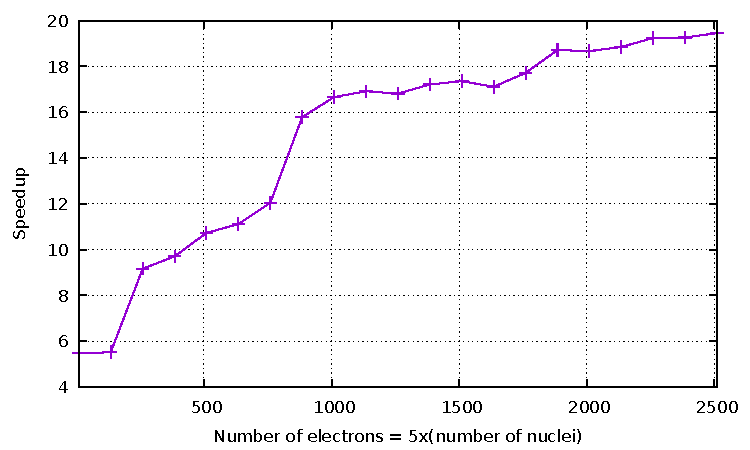
\includegraphics[width=0.75\textwidth]{speedup.pdf}
  \end{center}
  \caption{\label{fig:speedup}Speedup obtained after the re-expression of the three-body
    Jastrow factor.}
\end{figure}

This rewriting allowed us to move the computationally intensive part in
$\mathcal{O}(\Nat{\Nel}^2)$, i.e. the construction of the intermediate
tensors, into a BLAS3 matrix multiplication, the remaining part being
in $\mathcal{O}(\Nat \Nel)$.

The performance of the computation of the value, gradient and Laplacian of
the three-body Jastrow factor was measured on an Intel(R) Xeon(R) Gold
6130 processor, and the code was compiled with the Intel Fortran
compiler version 2021.1 with options
\mintinline{bash}{-O3 -xCORE-AVX512 -g -mkl=sequential -qopt-zmm-usage=high}.
The speedup with respect to the unoptimized kernel is presented in
figure~\ref{fig:speedup}, and reaches a factor of $19\times$ for the
largest system sizes. Performance analyzis of the mini-application
showed that at this stage we have reached 80\% of the single core peak
performance of the CPU core for this kernel. Profiling with MAQAO
confirmed the high quality of the code produced by our mini-application:
high array access efficiency, high arithmetic intensity, efficient
vectorization, and a large part of the time spent in the BLAS matrix
multiplication routines.

The same strategy of kernel extraction of the codes and rewriting
will be applied to all other possible computational bottlenecks of QMC
simulations, and then the kernels will be ready to be implemented in
the library.



\clearpage
\appendix
\section{Appendix: Documentation of the API}

In this section, we include as an example part of the documentation of
the library which is automatically generated from the {\orgmode}
files, in the current status. The rest of the documentation can be
found on the web site of the library\footnote{\url{https://trex-coe.github.io/qmckl}}.
Please, keep in mind that the library is still at an early development
stage. In the first six months, most of the efforts focused on
preparing solid bases for the development of
the library, more related to system programming than scientific
programming (the context variable, memory allocation, conventions,
Makefiles, generation of the documentation, \textit{etc}). The actual
implementation of the kernels is just starting.



